\section{FSM con registros de corrimiento \label{sec:s5}}

\begin{center}
	\begin{minipage}{12cm}
		\begin{tcolorbox}[title=Actividad 5]
			En ocasiones se puede resolver un problema utilizando un método diferente. ¿Se podrá resolver el problema utilizando dos registros de corrimiento de 4 bits?, ¿Uno para detectar los ceros y otros para detectar los unos consecutivos?, ¿Se podrá resolver con un solo registro de corrimiento? Compilar y simular.
		\end{tcolorbox}	
	\end{minipage}
\end{center}

\subsection{Dos registros de corrimiento}
La visualización RTL de la FSM, utilizando 2 registros de corrimiento, se muestra en la \autoref{fig:FSM_2SR_RTL}. El circuito hace uso de dos registros de 3 bits (el bit faltante corresponde al valor de W), dos comparadores, una compuerta OR y un registro a la salida para S.

Las simulaciones se visualizan en la \autoref{fig:FSM_2SR_Wave}. El comportamiento es el mismo que el descrito en actividades anteriores, siendo la única diferencia que se visualiza el corrimiento de bits en la simulación. Cuando el registro ``Zeros'' o ``Ones'' es exactamente igual a ``1111'', significa que hubo una secuencia de 4 ceros o 4 unos, consecutivos.

En los Anexos se localiza la descripción de la FSM utilizando 2 registros de corrimiento. Además de las entradas y salida, se declararon dos registros de 4 bits. En una lista sensible se detectan a los flancos de subida de CLK y de bajada de RST y dentro de esta se realiza el corrimiento de bits, de acuerdo al valor de la entrada W. Una vez que se detectan 4 valores consecutivos (ya sean unos o ceros), con una estructura \textit{if}, se pone la salida S en alto, de lo contrario, S estará en bajo.

\subsection{Un registro de corrimiento}
La visualización RTL de la FSM, utilizando un registro de corrimiento, se muestra en la \autoref{fig:FSM_1SR_RTL}. El circuito hace uso de un registro de 4 bits para corrimiento, un registro de 1 bit para la diferenciación de la secuencia de ceros y unos, dos multiplexores, un comparador y un registro a la salida para S.

Las simulaciones se visualizan en la \autoref{fig:FSM_1SR_Wave}. El comportamiento es el mismo que el descrito en actividades anteriores, siendo la única diferencia que se visualiza el corrimiento de bits en la simulación. Cuando el registro ``ZerosOnes'' es exactamente igual a ``1111'', significa que hubo una secuencia de 4 ceros o 4 unos, consecutivos.

En los Anexos se localiza la descripción de la FSM utilizando un registro de corrimiento. Además de las entradas y salida, se declaró un registro de 4 bits y otro registro para detectar si la secuencia es de ceros o de unos. En una lista sensible se detectan a los flancos de subida de CLK y de bajada de RST y dentro de esta se realiza el corrimiento de bits, de acuerdo al valor de la entrada W. El método difiere del circuito con 2 registros de corrimiento, debido a que, en lugar de usar un registro para detectar un tipo de secuencia, ahora se utiliza el mismo registro para detectar ambas secuencias, siendo el corrimiento hacia la izquierda para detectar unos y hacia la derecha para detectar ceros. Una vez que se detectan 4 valores consecutivos (ya sean unos o ceros), con una estructura \textit{if}, se pone la salida S en alto, de lo contrario, S estará en bajo.

\begin{figure}[ht]
	\centering
	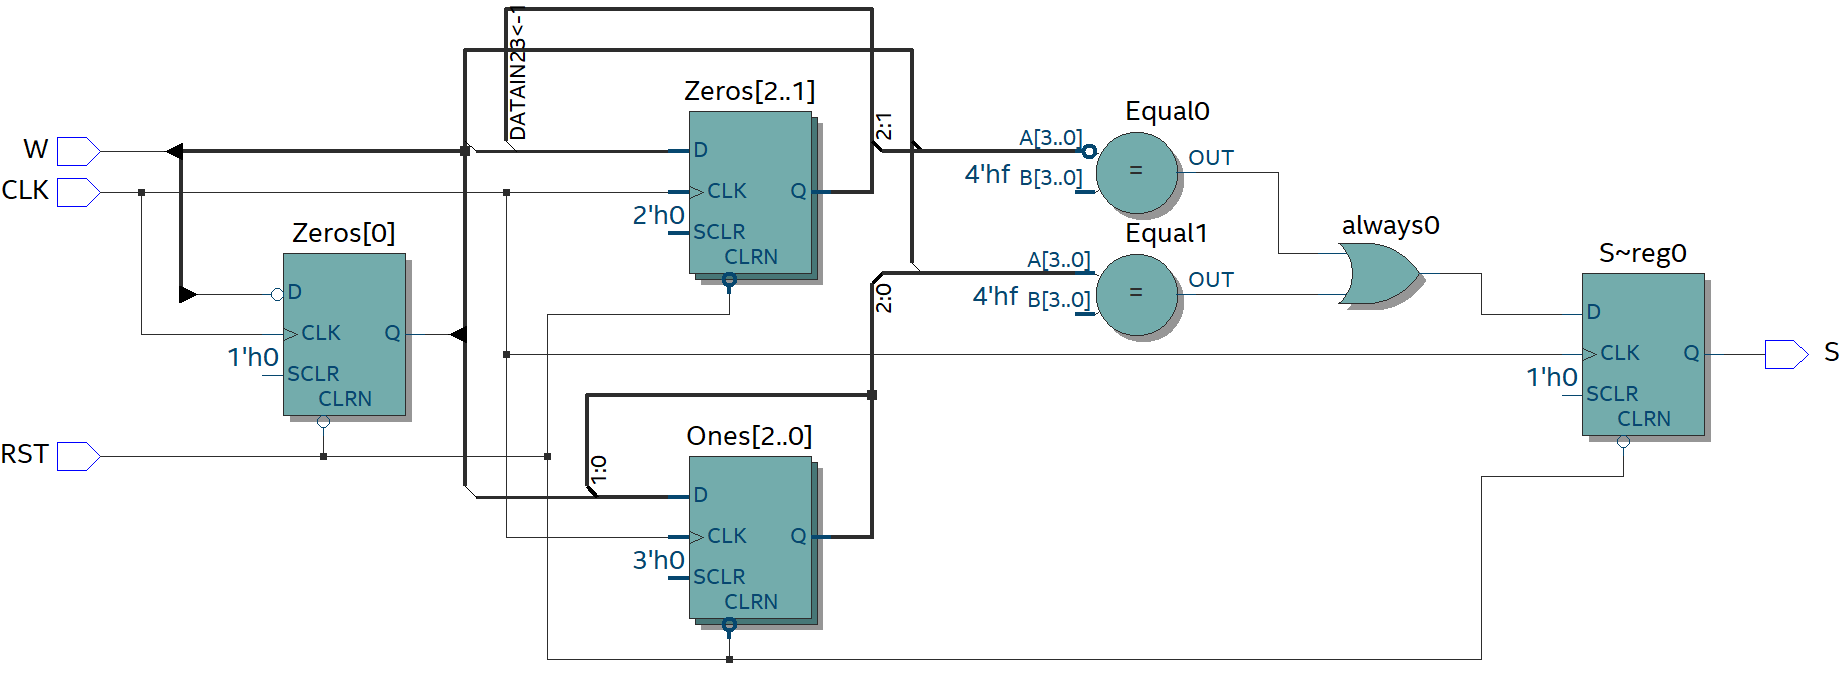
\includegraphics[scale=0.34]{FSM_2ShiftRegister_RTL.png}
	\caption{Diagrama RTL de la FSM, utilizando 2 registros de corrimiento. \label{fig:FSM_2SR_RTL}}
\end{figure}

\begin{figure}[ht]
	\centering
	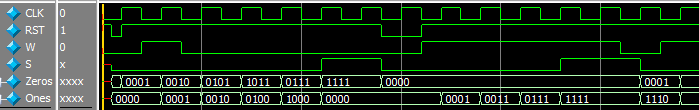
\includegraphics[scale=0.9]{FSM_2ShiftRegister_Wave.png}
	\caption{Simulación de la FSM, utilizando 2 registros de corrimiento, en el visor de formas de onda de ModelSim. \label{fig:FSM_2SR_Wave}}
\end{figure}

\begin{figure}[ht]
	\centering
	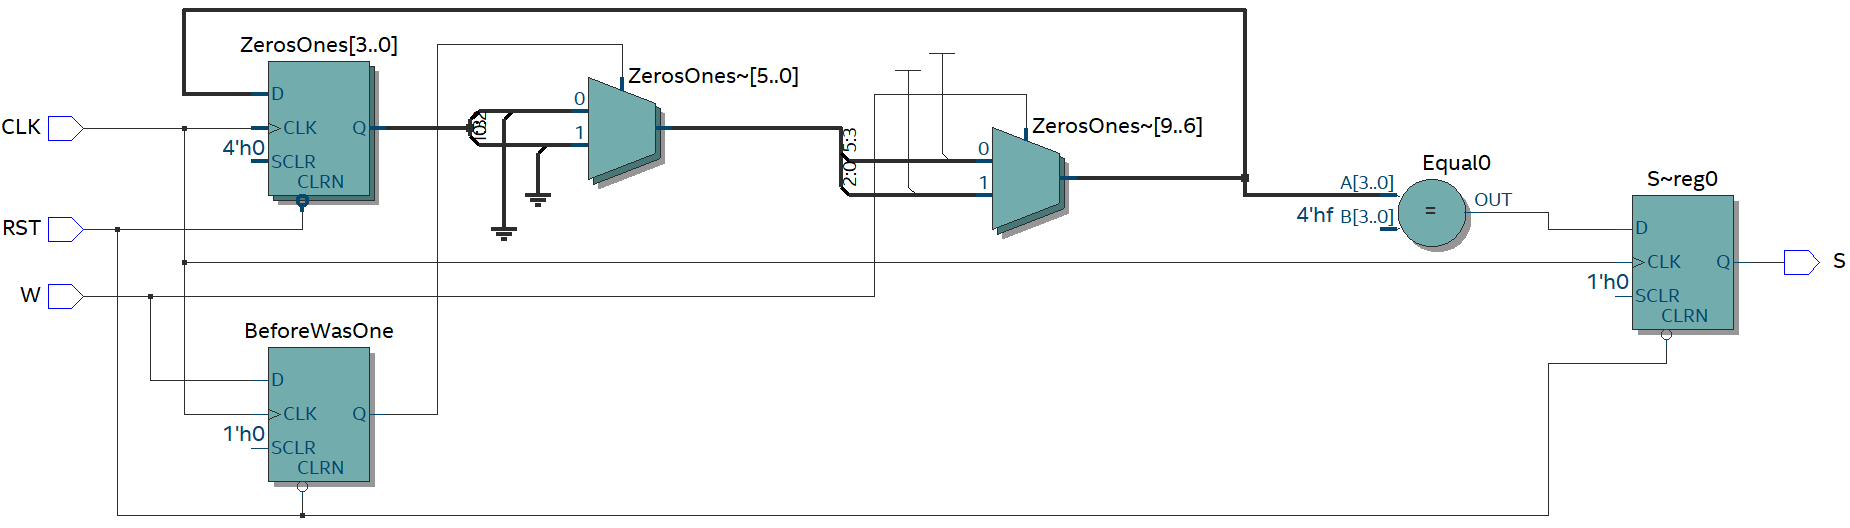
\includegraphics[scale=0.34]{FSM_1ShiftRegister_RTL.png}
	\caption{Diagrama RTL de la FSM, utilizando un solo registro de corrimiento. \label{fig:FSM_1SR_RTL}}
\end{figure}

\begin{figure}[ht]
	\centering
	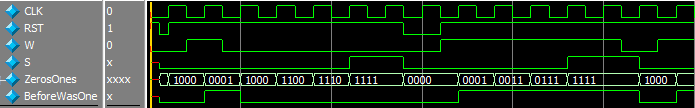
\includegraphics[scale=0.9]{FSM_1ShiftRegister_Wave.png}
	\caption{Simulación de la FSM, utilizando un solo registro de corrimiento, en el visor de formas de onda de ModelSim. \label{fig:FSM_1SR_Wave}}
\end{figure}